%==========================================================
\section{Mécanismes de contexte et optimisations mémoire}
%==========================================================

% --- Architecture ---
\begin{frame}{N threads utilisateur sur 1 thread noyau}
\centering
\begin{tikzpicture}[
  th/.style={draw, rounded corners=3pt, fill=blue!25, minimum width=1.5cm, minimum height=0.7cm, font=\small},
  arr/.style={->, >=Stealth, gray, thin},
]
  \node[th] (t1) at (0,    2.2) {Thread 1};
  \node[th] (t2) at (2.0,  2.2) {Thread 2};
  \node[th] (t3) at (4.0,  2.2) {Thread 3};
  \node[font=\Large, gray] at (5.6, 2.2) {$\cdots$};
  \node[th] (tn) at (7.0,  2.2) {Thread $n$};

  \node[draw, fill=orange!25, rounded corners=3pt,
        minimum width=8.5cm, minimum height=0.75cm, font=\small]
    (rq) at (3.5, 0.8) {\texttt{readyQueue}};

  \draw[arr] (t1.south) -- (rq.north);
  \draw[arr] (t2.south) -- (rq.north);
  \draw[arr] (t3.south) -- (rq.north);
  \draw[arr] (tn.south) -- (rq.north);

  \node[draw, fill=teal!20, rounded corners=3pt,
        minimum width=3.2cm, minimum height=0.75cm, font=\small]
    (kt) at (3.5, -0.7) {Thread noyau};

  \draw[->, very thick, blue!60] (rq.south) -- (kt.north)
    node[midway, right=5pt, font=\footnotesize] {ordonnanceur};

  \draw[dashed, gray!60] (-0.2, 0.1) -- (7.8, 0.1)
    node[right, font=\scriptsize\itshape] {frontière noyau};

  \node[font=\scriptsize\itshape, gray, align=right] at (-0.9, 2.2)  {espace\\utilisateur};
  \node[font=\scriptsize\itshape, gray]               at (-0.9, -0.7) {noyau};
\end{tikzpicture}
\end{frame}

% --- Context switch comparison ---
\begin{frame}{Changement de contexte}
\centering
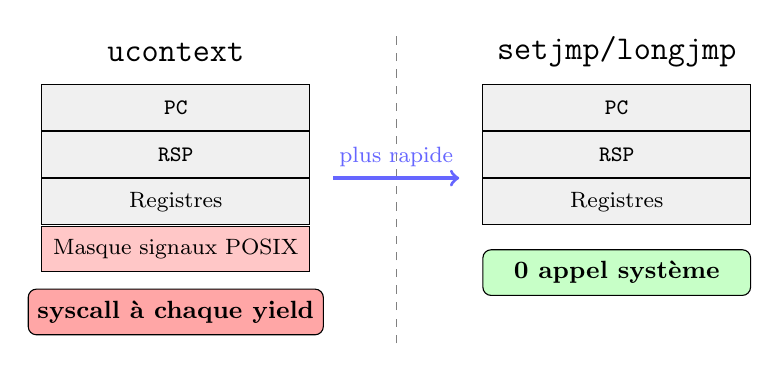
\begin{tikzpicture}[
  reg/.style={draw, fill=gray!12, minimum width=3.4cm, minimum height=0.58cm, font=\footnotesize},
  bad/.style={draw, fill=red!22,  minimum width=3.4cm, minimum height=0.58cm, font=\footnotesize},
  ok/.style ={draw, fill=green!22, rounded corners=3pt,
              minimum width=3.4cm, minimum height=0.58cm, font=\small\bfseries},
]
  % ucontext (left)
  \node[font=\large\bfseries]         at (-2.8,  2.3) {\texttt{ucontext}};
  \node[reg] (r1) at (-2.8,  1.6) {\texttt{PC}};
  \node[reg]      at (-2.8,  1.0) {\texttt{RSP}};
  \node[reg]      at (-2.8,  0.4) {Registres};
  \node[bad]      at (-2.8, -0.2) {Masque signaux POSIX};
  \node[draw, fill=red!35, rounded corners=3pt,
        minimum width=3.4cm, minimum height=0.58cm, font=\small\bfseries]
                  at (-2.8, -1.0) {syscall à chaque yield};

  % setjmp (right)
  \node[font=\large\bfseries]         at ( 2.8,  2.3) {\texttt{setjmp/longjmp}};
  \node[reg]      at ( 2.8,  1.6) {\texttt{PC}};
  \node[reg]      at ( 2.8,  1.0) {\texttt{RSP}};
  \node[reg]      at ( 2.8,  0.4) {Registres};
  \node[ok]       at ( 2.8, -0.5) {0 appel système};

  % separator + arrow
  \draw[dashed, gray] (0, -1.4) -- (0, 2.6);
  \draw[->, very thick, blue!60] (-0.8, 0.7) -- (0.8, 0.7)
    node[midway, above, font=\footnotesize] {plus rapide};
\end{tikzpicture}
\end{frame}

% --- Graphs context ---
\begin{frame}{Performances : \texttt{ucontext} vs \texttt{setjmp/longjmp}}
\begin{columns}[c]
  \column{0.5\textwidth}\centering
    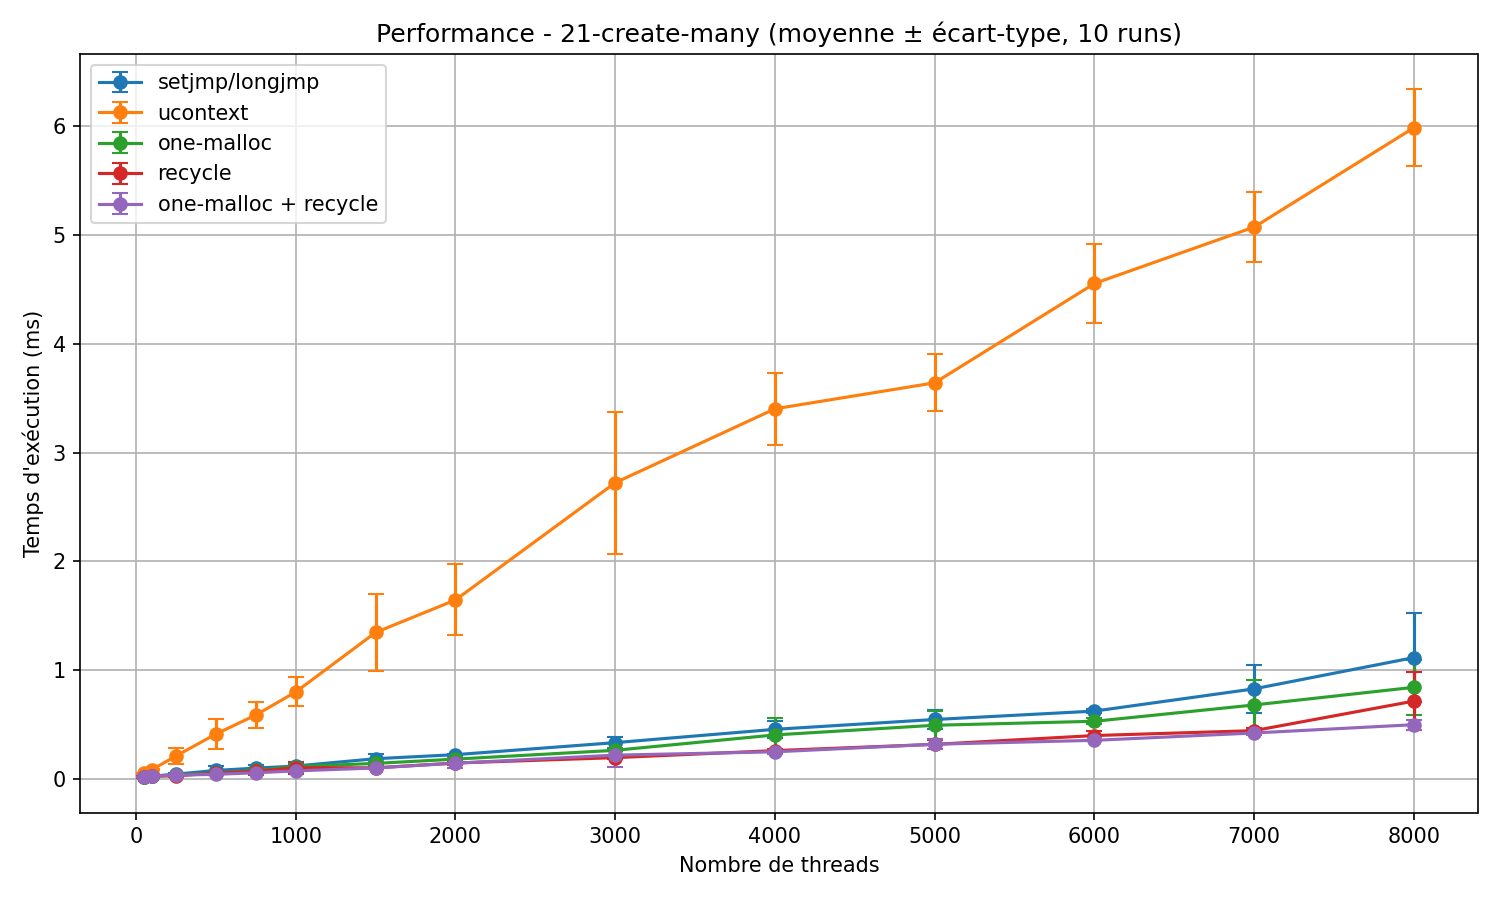
\includegraphics[width=\linewidth]{rapport-final/images/21-create-many-context.png}
    \\\small Création de $n$ threads
  \column{0.5\textwidth}\centering
    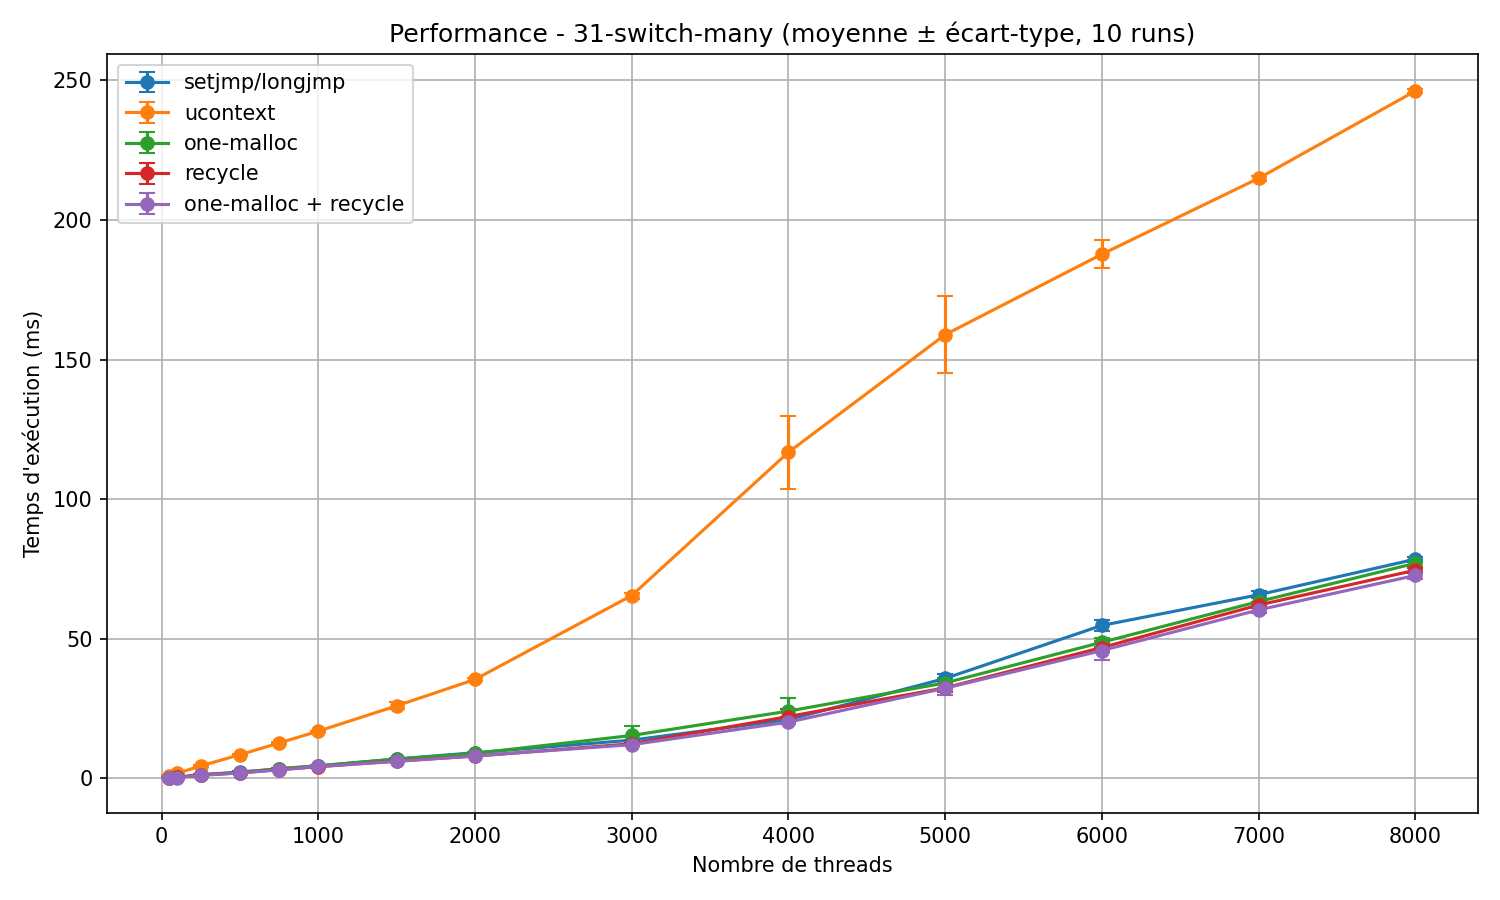
\includegraphics[width=\linewidth]{rapport-final/images/31-switch-many-context.png}
    \\\small $n \times 50$ changements de contexte
\end{columns}
\end{frame}

% --- Memory optimizations diagram ---
\begin{frame}{Optimisations mémoire : \texttt{one-malloc} et \texttt{recycle}}
\centering
\begin{tikzpicture}[
  blk/.style={draw, minimum height=0.65cm, font=\footnotesize},
  node distance=0pt,
  arr/.style={->, >=Stealth, thick, blue!60},
  box/.style={draw, rounded corners=3pt, minimum width=2.1cm,
              minimum height=0.65cm, font=\footnotesize},
]
  % --- one-malloc (top) ---
  \node[font=\small\bfseries] at (-3.5, 2.3) {Défaut};
  \node[blk, fill=blue!20, minimum width=1.8cm]  (sa) at (-4.2, 1.6) {\texttt{struct}};
  \node[blk, fill=orange!20, minimum width=1.8cm] (ska) at (-2.4, 1.6) {\texttt{stack}};
  \draw[<->, red!60, thin] (sa.east) -- (ska.west) node[midway, above, font=\tiny] {gap};

  \node[font=\small\bfseries] at ( 1.0, 2.3) {\texttt{USE\_ONE\_MALLOC}};
  \node[blk, fill=blue!20,   minimum width=1.8cm] (sb)  at (0.2,  1.6) {\texttt{struct}};
  \node[blk, fill=orange!20, minimum width=1.8cm] (skb) at (2.0,  1.6) {\texttt{stack}};
  \draw[green!60!black, thick] ($(sb.north west)+(-0.03,0.03)$)
    rectangle ($(skb.south east)+(0.03,-0.03)$);
  \node[font=\tiny, green!50!black] at (1.1, 1.2) {1 seul bloc};

  \draw[gray, dashed] (4.5, 0.9) -- (4.5, 2.6);

  % --- recycle (right of separator) ---
  \node[font=\small\bfseries] at (6.5, 2.3) {\texttt{USE\_RECYCLE}};

  \node[box, fill=blue!20]   (cr)  at (5.5, 1.4) {\texttt{create}};
  \node[box, fill=teal!20]   (run) at (7.5, 1.4) {\texttt{run}};
  \node[box, fill=green!20]  (jo)  at (7.5, 0.2) {\texttt{join}};
  \node[box, fill=orange!25] (fq)  at (5.5, 0.2) {\texttt{freeQueue}};

  \draw[arr] (cr)  -- (run);
  \draw[arr] (run) -- (jo);
  \draw[arr] (jo)  -- (fq)  node[midway, below, font=\tiny] {recycle};
  \draw[arr] (fq)  -- (cr)  node[midway, left,  font=\tiny] {réutilise};

  % separator line between one-malloc and recycle
  \draw[gray, dashed] (-0.5, -0.4) -- (8.5, -0.4);
  \node[font=\footnotesize\itshape, gray] at (4, -0.75)
    {Combinaison \texttt{one-malloc + recycle} = version la plus rapide};
\end{tikzpicture}
\end{frame}

% --- Graphs optim ---
\begin{frame}{Performances des optimisations}
\begin{columns}[c]
  \column{0.5\textwidth}\centering
    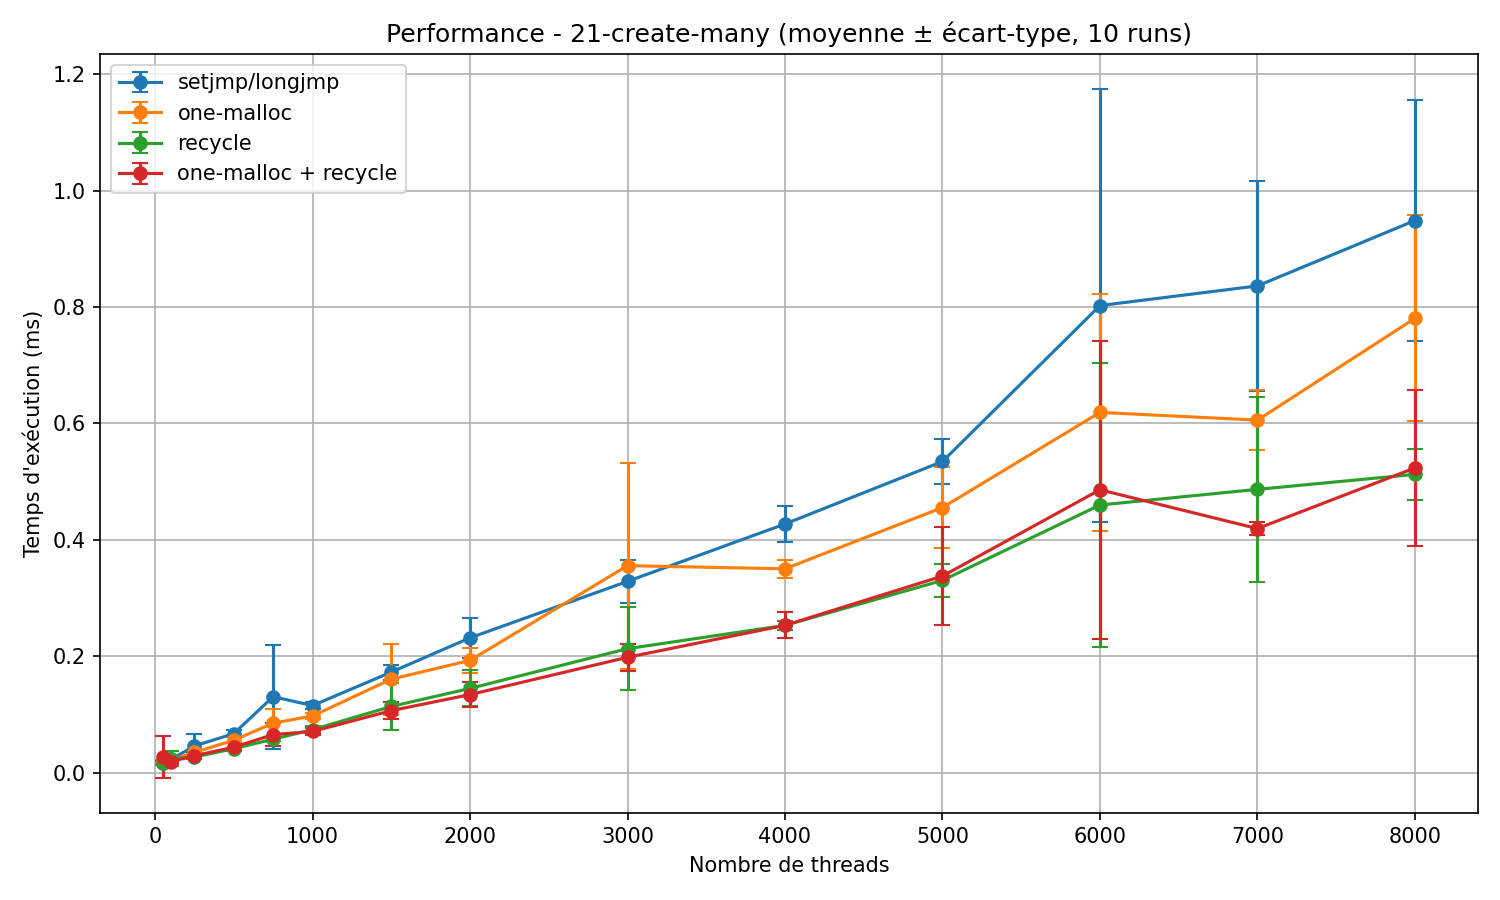
\includegraphics[width=\linewidth]{rapport-final/images/21-create-many-optim.png}
    \\\small Création de $n$ threads
  \column{0.5\textwidth}\centering
    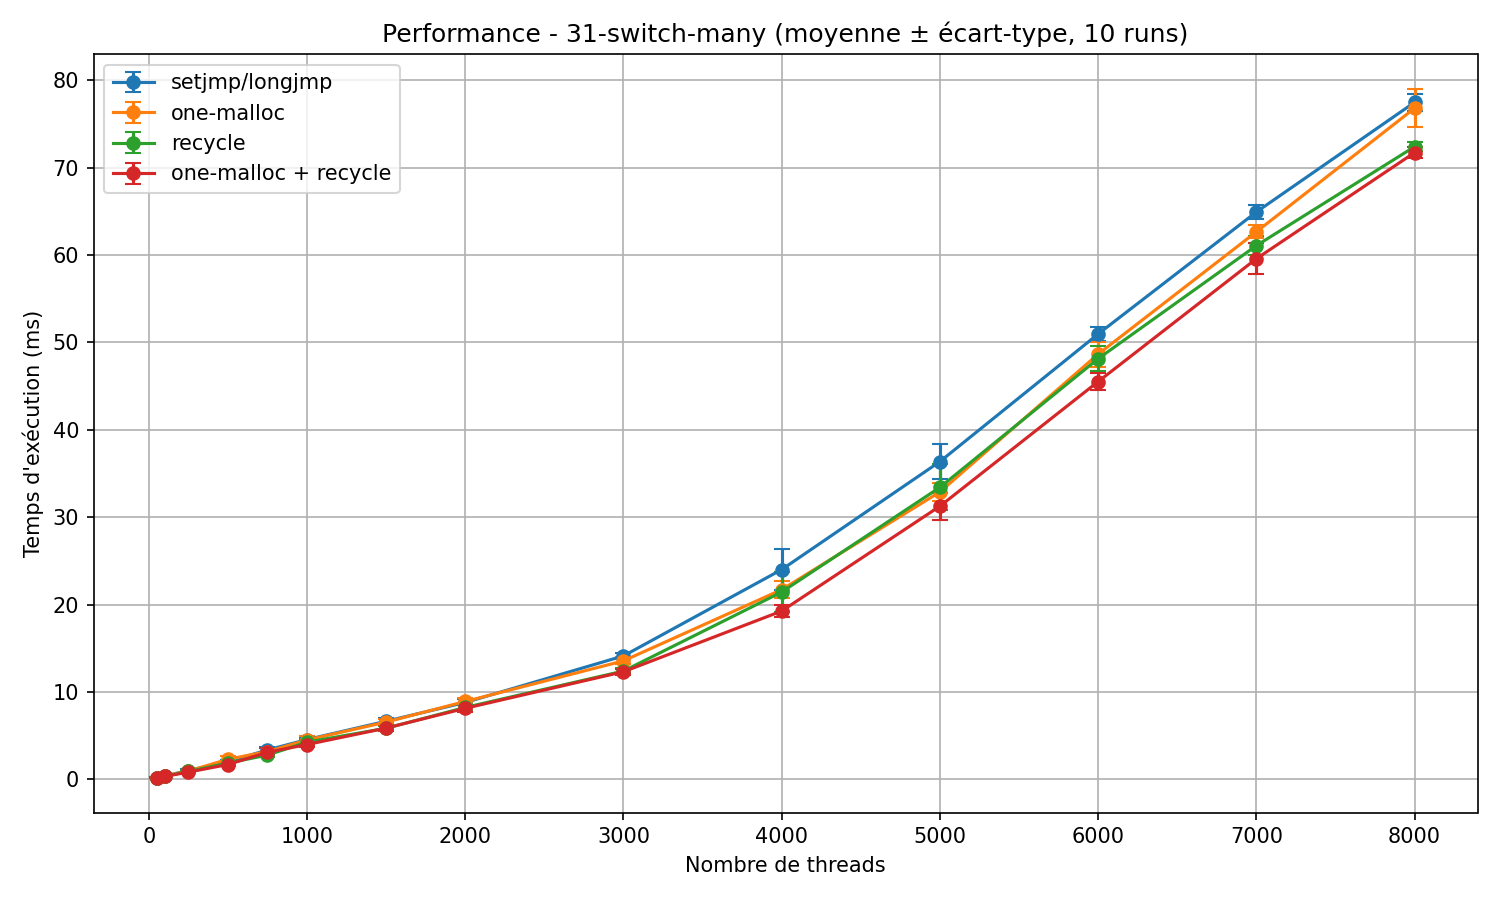
\includegraphics[width=\linewidth]{rapport-final/images/31-switch-many-optim.png}
    \\\small $n \times 50$ changements de contexte
\end{columns}
\vspace{0.3em}
\centering\small
\textbf{recycle} = gain dominant \quad
\textbf{yields} = non affectés (pas d'allocation)
\end{frame}
